\documentclass[dvipdfmx]{jsarticle}
\setcounter{section}{3}
\setcounter{subsection}{2}
\usepackage{xr}
\externaldocument{1.3.2}
\externaldocument{1.2.7}
\usepackage{amsmath,amsfonts,amssymb,array,comment,mathtools,url,docmute}
\usepackage{longtable,booktabs,dcolumn,tabularx,mathtools,multirow,colortbl,xcolor}
\usepackage[dvipdfmx]{graphics}
\usepackage{bmpsize}
\usepackage{amsthm}
\usepackage{enumitem}
\setlistdepth{20}
\renewlist{itemize}{itemize}{20}
\setlist[itemize]{label=•}
\renewlist{enumerate}{enumerate}{20}
\setlist[enumerate]{label=\arabic*.}
\setcounter{MaxMatrixCols}{20}
\setcounter{tocdepth}{3}
\newcommand{\rotin}{\text{\rotatebox[origin=c]{90}{$\in $}}}
\renewcommand{\thesection}{第\arabic{section}部}
\renewcommand{\thesubsection}{\arabic{section}.\arabic{subsection}}
\renewcommand{\thesubsubsection}{\arabic{section}.\arabic{subsection}.\arabic{subsubsection}}
\everymath{\displaystyle}
\allowdisplaybreaks[4]
\usepackage{vtable}
\theoremstyle{definition}
\newtheorem{thm}{定理}[subsection]
\newtheorem*{thm*}{定理}
\newtheorem{dfn}{定義}[subsection]
\newtheorem*{dfn*}{定義}
\newtheorem{axs}[dfn]{公理}
\newtheorem*{axs*}{公理}
\renewcommand{\headfont}{\bfseries}
\makeatletter
  \renewcommand{\section}{%
    \@startsection{section}{1}{\z@}%
    {\Cvs}{\Cvs}%
    {\normalfont\huge\headfont\raggedright}}
\makeatother
\makeatletter
  \renewcommand{\subsection}{%
    \@startsection{subsection}{2}{\z@}%
    {0.5\Cvs}{0.5\Cvs}%
    {\normalfont\LARGE\headfont\raggedright}}
\makeatother
\makeatletter
  \renewcommand{\subsubsection}{%
    \@startsection{subsubsection}{3}{\z@}%
    {0.4\Cvs}{0.4\Cvs}%
    {\normalfont\Large\headfont\raggedright}}
\makeatother
\makeatletter
\renewenvironment{proof}[1][\proofname]{\par
  \pushQED{\qed}%
  \normalfont \topsep6\p@\@plus6\p@\relax
  \trivlist
  \item\relax
  {
  #1\@addpunct{.}}\hspace\labelsep\ignorespaces
}{%
  \popQED\endtrivlist\@endpefalse
}
\makeatother
\renewcommand{\proofname}{\textbf{証明}}
\usepackage{tikz,graphics}
\usepackage[dvipdfmx]{hyperref}
\usepackage{pxjahyper}
\hypersetup{
 setpagesize=false,
 bookmarks=true,
 bookmarksdepth=tocdepth,
 bookmarksnumbered=true,
 colorlinks=false,
 pdftitle={},
 pdfsubject={},
 pdfauthor={},
 pdfkeywords={}}
\begin{document}
%\hypertarget{zornux306eux88dcux984c}{%
\subsection{Zornの補題}%\label{zornux306eux88dcux984c}}
%\hypertarget{ux6574ux5217ux96c6ux5408ux306bux95a2ux3059ux308bux4e00ux547dux984c}{%
\subsubsection{整列集合に関する一命題}%\label{ux6574ux5217ux96c6ux5408ux306bux95a2ux3059ux308bux4e00ux547dux984c}}
\begin{thm}\label{1.3.3.1}
集合$W$の部分集合族$\left\{ W_{\lambda} \right\}_{\lambda \in \varLambda }$が与えられて、$\forall\lambda \in \varLambda $に対し、その組$\left( W_{\lambda},O_{\lambda} \right)$が整列集合をなし、$\forall\lambda,\mu \in \varLambda $に対し、$\lambda \neq \mu$が成り立つなら、それらの集合たち$W_{\lambda}$、$W_{\mu}$のうちどちらか一方が他方の切片となっているとする。このとき、$\forall a,b \in \bigcup_{\lambda \in \varLambda } W_{\lambda}$に対し、$a,b \in W_{\lambda}$が成り立つようなその添数集合$\varLambda $の元$\lambda$が存在する。このとき、$aO_{\lambda}b$または$bO_{\lambda}a$に応じて$aOb$、$bOa$と定義すると、その関係$O$はその添数$\lambda$によらなくその組$\left( \bigcup_{\lambda \in \varLambda } W_{\lambda},O \right)$は整列集合となる。さらに、$\forall\lambda \in \varLambda $に対し、その整列集合$\left( W_{\lambda},O_{\lambda} \right)$はその整列集合$\left( \bigcup_{\lambda \in \varLambda } W_{\lambda},O \right)$自身であるか、その集合$\bigcup_{\lambda \in \varLambda } W_{\lambda}$の切片$W'$を用いた整列集合$\left( W',O \right)$である。
\end{thm}
\begin{proof}
集合$W$の部分集合族$\left\{ W_{\lambda} \right\}_{\lambda \in \varLambda }$が与えられて、$\forall\lambda \in \varLambda $に対し、その組$\left( W_{\lambda},O_{\lambda} \right)$が整列集合をなし、$\forall\lambda,\mu \in \varLambda $に対し、$\lambda \neq \mu$が成り立つなら、それらの集合たち$W_{\lambda}$、$W_{\mu}$のうちどちらか一方が他方の切片となっているとする。このとき、$\forall a,b \in \bigcup_{\lambda \in \varLambda } W_{\lambda}$に対し、$a \in W_{\lambda}$かつ$b \in W_{\mu}$なる添数たち$\lambda$、$\mu$がその添数集合$\varLambda $に存在することになる。$\lambda = \mu$のとき、$a,b \in W_{\lambda}$が成り立つようなその添数集合$\varLambda $の元$\lambda$が存在することがいえている。$\lambda \neq \mu$のとき、仮定よりそれらの集合たち$W_{\lambda}$、$W_{\mu}$のうちどちらか一方が他方の切片となっているので、その集合$W_{\mu}$がその集合$W_{\lambda}$の切片となっていると仮定しても一般性は失われない。したがって、$W_{\mu} \subseteq W_{\lambda}$が成り立ち$a,b \in W_{\lambda}$が得られる。したがって、$a,b \in W_{\lambda}$が成り立つようなその添数集合$\varLambda $の元$\lambda$が存在することがいえている。\par
このとき、$aO_{\lambda}b$または$bO_{\lambda}a$に応じて$aOb$、$bOa$と定義すると、$a,b \in W_{\lambda}$かつ$a,b \in W_{\mu}$なる互いに異なる添数$\lambda$、$\mu$が与えられたとすれば、仮定よりそれらの集合たち$W_{\lambda}$、$W_{\mu}$のうちどちらか一方が他方の切片となっているのであったので、その集合$W_{\mu}$がその集合$W_{\lambda}$の切片となっていると仮定しても一般性は失われない。したがって、その整列集合$\left( W_{\mu},O_{\mu} \right)$はその整列集合$\left( W_{\lambda},O_{\lambda} \right)$の部分順序集合となっているので、$aO_{\lambda}b$と$aO_{\mu}b$、あるいは、$bO_{\lambda}a$と$bO_{\mu}a$とは同値である。したがって、その関係$O$はその添数$\lambda$によらない。\par
$a,b,c \in \bigcup_{\lambda \in \varLambda } W_{\lambda}$が成り立つとすれば、上記の議論により$a,b,c \in W_{\lambda}$が成り立つような添数$\lambda$がその添数集合$\varLambda $に存在する。このとき、その組$\left( W_{\lambda},O_{\lambda} \right)$は整列集合であるので、次のことが成り立つ。
\begin{itemize}
\item
  $\forall a \in W_{\lambda}$に対し、$aO_{\lambda}a$が成り立つ。
\item
  $\forall a,b \in W_{\lambda}$に対し、$aO_{\lambda}b \land bO_{\lambda}a \Rightarrow a = b$が成り立つ。
\item
  $\forall a,b,c \in W_{\lambda}$に対し、$aO_{\lambda}b \land bO_{\lambda}c \Rightarrow aO_{\lambda}c$が成り立つ。
\end{itemize}
これにより、次のことが成り立つ。
\begin{itemize}
\item
  $\forall a \in \bigcup_{\lambda \in \varLambda } W_{\lambda}$に対し、$aOa$が成り立つ。
\item
  $\forall a,b \in \bigcup_{\lambda \in \varLambda } W_{\lambda}$に対し、$aOb \land bOa \Rightarrow a = b$が成り立つ。
\item
  $\forall a,b,c \in \bigcup_{\lambda \in \varLambda } W_{\lambda}$に対し、$aOb \land bOc \Rightarrow aOc$が成り立つ。
\end{itemize}
以上より、その組$\left( \bigcup_{\lambda \in \varLambda } W_{\lambda},O \right)$は順序集合となる。\par
その集合$\bigcup_{\lambda \in \varLambda } W_{\lambda}$の空集合でない任意の部分集合$W'$が考えられれば、$W' \neq \emptyset$より$a \in W' \subseteq \bigcup_{\lambda \in \varLambda } W_{\lambda}$が成り立つ。上記の議論により$a \in W_{\lambda}$なる添数$\lambda$がその添数集合$\varLambda $に存在するので、$W' \cap W_{\lambda} = \emptyset$なる添数$\lambda$がその添数集合$\varLambda $に存在することがいえる。このとき、その組$\left( W_{\lambda},O_{\lambda} \right)$は整列集合であるから、その集合$W' \cap W_{\lambda}$はその集合$W_{\lambda}$の部分集合でありその組$\left( W' \cap W_{\lambda},O_{\lambda} \right)$もまた整列集合であるから、その最小元$\min\left( W' \cap W_{\lambda} \right)$がその集合$W' \cap W_{\lambda}$に存在する。ここで、$\forall a \in W'$に対し、$a \in W_{\lambda}$のとき、$a \in W' \cap W_{\lambda}$が成り立つので、$\min\left( W' \cap W_{\lambda} \right)O_{\lambda}a$が成り立つ。$a \notin W_{\lambda}$のとき、$a \in W_{\lambda'}$なる添数$\lambda'$がその添数集合$\varLambda $に存在し、$W_{\lambda'} \subseteq W_{\lambda}$が成り立つと仮定すると、$a \in W_{\lambda}$が得られ矛盾するので、$W_{\lambda} \subset W_{\lambda'}$が成り立ち、仮定よりその集合$W_{\lambda}$がその集合$W_{\lambda'}$の切片である。ここで、$aO_{\lambda'}\min\left( W' \cap W_{\lambda} \right)$かつ$\min\left( W' \cap W_{\lambda} \right) \neq a$が成り立つと仮定すると、$\min\left( W' \cap W_{\lambda} \right) \in W_{\lambda}$であるから、切片の定義より$a \in W_{\lambda}$が成り立つことになり、これは$a \notin W_{\lambda}$が成り立つことに矛盾する。したがって、$\min\left( W' \cap W_{\lambda} \right)O_{\lambda'}a$が成り立つ。以上の場合でも、$\forall a \in W'$に対し、$\min\left( W' \cap W_{\lambda} \right)O_{\lambda'}a$が成り立つので、$\min\left( W' \cap W_{\lambda} \right) = \min W'$が成り立つ。以上より、その順序集合$\left( \bigcup_{\lambda \in \varLambda } W_{\lambda},O \right)$は整列集合である。\par
さらに、$\forall\lambda \in \varLambda $に対し、その整列集合$\left( W_{\lambda},O_{\lambda} \right)$がその整列集合$\left( \bigcup_{\lambda \in \varLambda } W_{\lambda},O \right)$と一致することはあり得る。一方で、その整列集合$\left( W_{\lambda},O_{\lambda} \right)$がその整列集合$\left( \bigcup_{\lambda \in \varLambda } W_{\lambda},O \right)$と一致しないとき、$W_{\lambda} \subset \bigcup_{\lambda \in \varLambda } W_{\lambda}$が成り立つことになり、その整列集合$\left( W_{\lambda},O_{\lambda} \right)$はその整列集合$\left( \bigcup_{\lambda \in \varLambda } W_{\lambda},O \right)$の部分順序集合である。このとき、$a \in W_{\lambda}$かつ$b \in \bigcup_{\lambda \in \varLambda } W_{\lambda}$かつ$bOa$かつ$a \neq b$が成り立つと仮定すると、$a,b \in W_{\lambda'}$なる添数$\lambda'$がその添数集合$\varLambda $に存在する。ここで、$W_{\lambda} = W_{\lambda'}$が成り立つとき、または、その集合$W_{\lambda'}$がその集合$W_{\lambda}$の切片であるとき、$b \in W_{\lambda}$が得られる。その集合$W_{\lambda}$がその集合$W_{\lambda'}$の切片であるとき、$bO_{\lambda'}a$かつ$a \neq b$が成り立つので、やはり$b \in W_{\lambda}$が得られる。以上の場合でも、$b \in W_{\lambda}$が成り立つので、定理\ref{1.3.2.11}よりその集合$W_{\lambda}$はその集合$\bigcup_{\lambda \in \varLambda } W_{\lambda}$の切片である。この切片を$W'$とおくと、その整列集合$\left( W_{\lambda},O_{\lambda} \right)$は整列集合$\left( W',O \right)$となる。以上より、$\forall\lambda \in \varLambda $に対し、その整列集合$\left( W_{\lambda},O_{\lambda} \right)$はその整列集合$\left( \bigcup_{\lambda \in \varLambda } W_{\lambda},O \right)$自身であるか、その集合$\bigcup_{\lambda \in \varLambda } W_{\lambda}$の切片$W'$を用いた整列集合$\left( W',O \right)$である。\par
よって、$\forall a,b \in \bigcup_{\lambda \in \varLambda } W_{\lambda}$に対し、$a,b \in W_{\lambda}$が成り立つようなその添数集合$\varLambda $の元$\lambda$が存在する。このとき、$aO_{\lambda}b$または$bO_{\lambda}a$に応じて$aOb$、$bOa$と定義すると、その関係$O$はその添数$\lambda$によらなくその組$\left( \bigcup_{\lambda \in \varLambda } W_{\lambda},O \right)$は整列集合となる。さらに、$\forall\lambda \in \varLambda $に対し、その整列集合$\left( W_{\lambda},O_{\lambda} \right)$はその整列集合$\left( \bigcup_{\lambda \in \varLambda } W_{\lambda},O \right)$自身であるか、その集合$\bigcup_{\lambda \in \varLambda } W_{\lambda}$の切片$W'$を用いた整列集合$\left( W',O \right)$である。
\end{proof}
\begin{thm}\label{1.3.3.2}
集合$W$の部分集合族$\left\{ W_{\lambda} \right\}_{\lambda \in \varLambda }$が与えられて、$\forall\lambda \in \varLambda $に対し、その組$\left( W_{\lambda},O_{\lambda} \right)$が順序集合$(W,O)$の部分順序集合として整列集合をなし、$\forall\lambda,\mu \in \varLambda $に対し、$\lambda \neq \mu$が成り立つなら、それらの集合たち$W_{\lambda}$、$W_{\mu}$のうちどちらか一方が他方の切片となっているとする。このとき、その組$\left( \bigcup_{\lambda \in \varLambda } W_{\lambda},O \right)$はその順序集合$(W,O)$の部分順序集合として整列集合となる。さらに、$\forall\lambda \in \varLambda $に対し、その整列集合$\left( W_{\lambda},O_{\lambda} \right)$はその整列集合$\left( \bigcup_{\lambda \in \varLambda } W_{\lambda},O \right)$自身であるか、その集合$\bigcup_{\lambda \in \varLambda } W_{\lambda}$の切片$W'$を用いた整列集合$\left( W',O \right)$である。
\end{thm}
\begin{proof}
集合$W$の部分集合族$\left\{ W_{\lambda} \right\}_{\lambda \in \varLambda }$が与えられて、$\forall\lambda \in \varLambda $に対し、その組$\left( W_{\lambda},O_{\lambda} \right)$が順序集合$(W,O)$の部分順序集合として整列集合をなし、$\forall\lambda,\mu \in \varLambda $に対し、$\lambda \neq \mu$が成り立つなら、それらの集合たち$W_{\lambda}$、$W_{\mu}$のうちどちらか一方が他方の切片となっているとする。このとき、上記の定理\ref{1.3.3.1}より、$aO_{\lambda}b$または$bO_{\lambda}a$に応じて$aOb$、$bOa$と同値としても、その関係$O$はその添数$\lambda$によらなくその組$\left( \bigcup_{\lambda \in \varLambda } W_{\lambda},O \right)$は整列集合となる。さらに、$\forall\lambda \in \varLambda $に対し、その整列集合$\left( W_{\lambda},O_{\lambda} \right)$はその整列集合$\left( \bigcup_{\lambda \in \varLambda } W_{\lambda},O \right)$自身であるか、その集合$\bigcup_{\lambda \in \varLambda } W_{\lambda}$の切片$W'$を用いた整列集合$\left( W',O \right)$である。ここで、$\bigcup_{\lambda \in \varLambda } W_{\lambda} \subseteq W$が成り立つので、その整列集合$\left( \bigcup_{\lambda \in \varLambda } W_{\lambda},O \right)$はその順序集合$(W,O)$の部分順序集合でもある。よって、その組$\left( \bigcup_{\lambda \in \varLambda } W_{\lambda},O \right)$はその順序集合$(W,O)$の部分順序集合として整列集合となる。さらに、$\forall\lambda \in \varLambda $に対し、その整列集合$\left( W_{\lambda},O_{\lambda} \right)$はその整列集合$\left( \bigcup_{\lambda \in \varLambda } W_{\lambda},O \right)$自身であるか、その集合$\bigcup_{\lambda \in \varLambda } W_{\lambda}$の切片$W'$を用いた整列集合$\left( W',O \right)$である。
\end{proof}
%\hypertarget{zornux306eux88dcux984c-1}{%
\subsubsection{Zornの補題}%\label{zornux306eux88dcux984c-1}}
\begin{dfn}
順序集合$(A,O)$が与えられたとき、その任意の空集合でないかつ全順序な部分順序集合$\left( A',O \right)$の上限$\sup A'$がその集合$A$に存在するとき、その順序集合$(A,O)$は帰納的であるという。
\end{dfn}
\begin{thm}\label{1.3.3.3}
帰納的な順序集合$(A,O)$が与えられたとき、$\forall a \in A$に対し、$aO\varphi(a)$が成り立つような写像$\varphi:A \rightarrow A$が考えられると、$\varphi(a) = a$となるような元$a$がその集合$A$に存在する。
\end{thm}
\begin{proof}
帰納的な順序集合$(A,O)$が与えられたとき、$\forall a \in A$に対し、$aO\varphi(a)$が成り立つような写像$\varphi:A \rightarrow A$が考えられるとする。このとき、その集合$A$のある元$a'$を用いて次のことが成り立つようなその集合$A$の部分集合$A'$が考えられると、
\begin{itemize}
\item
  その組$\left( A',O \right)$はその順序集合$(A,O)$の部分順序集合として整列集合となる。
\item
  $a' = \min A'$が成り立つ。
\item
  その集合$A'$の元$a$の直前の元$a_{*}$がその集合$A'$に存在するなら、$\varphi\left( a_{*} \right) = a$が成り立つ。
\item
  その元$a'$でないその集合$A'$の元$a$の直前の元がその集合$A'$に存在しないなら、その集合$A'$のその元$a$による切片${A'}_{Oa}$のその順序集合$(A,O)$における上限$\sup{A'}_{Oa}$はその元$a$に等しい。
\end{itemize}
そのような部分集合$A'$は存在する。例えば、$\left\{ a' \right\}$などが挙げられる。このような部分集合$A'$全体の集合を$\mathfrak{W}$とおくと、その集合$\mathfrak{W}$は空集合でない。\par
ここで、$\forall V,W\in \mathfrak{W}$に対し、2つの整列集合たち$(V,O)$、$(W,O)$がこれによって与えられ、整列集合の比較定理より$(V,O) \simeq (W,O)$が成り立つか、どちらか一方が他方のある切片と順序同型である。\par
その整列集合$(V,O)$がその整列集合$(W,O)$と順序同型であるとき、その順序同型写像を$f$とおくと、仮定より次式が成り立つことから、
\begin{align*}
a' = \min V = \min W
\end{align*}
$f\left( \min V \right) = \min V$が得られる。次に、その元$a'$でないその集合$V$の任意の元$a$によるその集合$V$の切片$V_{Oa}$の任意の元$b$に対し、$f(b) = b$が成り立つと仮定すると、その元$a$の直前の元$a_{*}$がその集合$V$に存在するなら、その写像$f$が順序同型写像なので、その元$f\left( a_{*} \right)$がその集合$W$でのその元$f(a)$の直前の元となる。このとき、$a_{*} \in V_{Oa}$が成り立つので、仮定より$f\left( a_{*} \right) = a_{*}$が成り立ち、仮定より次式が成り立つ。
\begin{align*}
f(a) = \varphi\left( f\left( a_{*} \right) \right) = \varphi\left( a_{*} \right) = a
\end{align*}
その元$a$の直前の元$a_{*}$がその集合$V$に存在しないなら、その写像$f$が順序同型写像なので、その集合$W$にその元$f(a)$の直前の元が存在しないことになるかつ、$\forall a'' \in V_{Oa}$に対し、$a''Oa$かつ$a \neq a''$が成り立つので、$f\left( a'' \right)Of(a)$かつ$f(a) \neq f\left( a'' \right)$が成り立ち、したがって、$V\left( f|V_{Oa} \right) \subseteq W_{Of(a)}$が成り立つ。逆に、$\forall a'' \in W_{Of(a)}$に対し、$a''Of(a)$かつ$f(a) \neq a''$が成り立つので、その写像$f$が順序同型写像であることに注意すると、$f^{- 1}\left( a'' \right)Oa$かつ$a \neq f^{- 1}\left( a'' \right)$が成り立ち、したがって、$f^{- 1}\left( a'' \right) \in V_{Oa}$が得られ、$a'' = f\left( f^{- 1}\left( a'' \right) \right) \in V\left( f|V_{Oa} \right)$が成り立つので、$V\left( f|V_{Oa} \right) \supseteq W_{Of(a)}$が成り立つ。以上、$V\left( f|V_{Oa} \right) = W_{Of(a)}$が得られる。ここで、$\forall b \in V_{Oa}$に対し、$f(b) = b$が成り立つので、$V_{Oa} = W_{Of(a)}$が成り立ち、したがって、仮定より次式が成り立つ。
\begin{align*}
f(a) = \sup W_{Of(a)} = \sup V_{Oa} = a
\end{align*}
以上より、超限帰納法により$\forall a \in W$に対し、$f(a) = a$が成り立つので、$V = W$が成り立つ。\par
その整列集合$(V,O)$がその集合$W$のある切片$W_{Ob'}$を用いた整列集合$\left( W_{Ob'},O \right)$と順序同型であるとき、その順序同型写像を$f$とおくと、仮定より次式が成り立つことから、
\begin{align*}
a' = \min V = \min W = \min W_{Ob'}
\end{align*}
$f\left( \min V \right) = \min V$が得られる。次に、その元$a'$でないその集合$V$の任意の元$a$によるその集合$V$の切片$V_{Oa}$の任意の元$b$に対し、$f(b) = b$が成り立つと仮定すると、その元$a$の直前の元$a_{*}$がその集合$V$に存在するなら、その写像$f$が順序同型写像なので、その元$f\left( a_{*} \right)$がその集合$W_{Ob'}$でのその元$f(a)$の直前の元となる。このとき、$a_{*} \in V_{Oa}$が成り立つので、仮定より$f\left( a_{*} \right) = a_{*}$が成り立ち、仮定より次式が成り立つ。
\begin{align*}
f(a) = \varphi\left( f\left( a_{*} \right) \right) = \varphi\left( a_{*} \right) = a
\end{align*}
その元$a$の直前の元$a_{*}$がその集合$V$に存在しないなら、その写像$f$が順序同型写像なので、その集合$W_{Ob'}$に、即ち、その集合$W$にその元$f(a)$の直前の元が存在しないことになるかつ、$\forall a'' \in V_{Oa}$に対し、$a''Oa$かつ$a \neq a''$が成り立つので、$f\left( a'' \right)Of(a)$かつ$f(a) \neq f\left( a'' \right)$が成り立ち、したがって、$V\left( f|V_{Oa} \right) \subseteq {W_{Ob'}}_{Of(a)}$が成り立つ。逆に、$\forall a'' \in {W_{Ob'}}_{Of(a)}$に対し、$a''Of(a)$かつ$f(a) \neq a''$が成り立つので、その写像$f$が順序同型写像であることに注意すると、$f^{- 1}\left( a'' \right)Oa$かつ$a \neq f^{- 1}\left( a'' \right)$が成り立ち、したがって、$f^{- 1}\left( a'' \right) \in V_{Oa}$が得られ、$a'' = f\left( f^{- 1}\left( a'' \right) \right) \in V\left( f|V_{Oa} \right)$が成り立つので、$V\left( f|V_{Oa} \right) \supseteq {W_{Ob'}}_{Of(a)}$が成り立つ。また、定理\ref{1.3.2.14}に注意すれば、以上より$V\left( f|V_{Oa} \right) = {W_{Ob'}}_{Of(a)} = W_{Of(a)}$が得られる。ここで、$\forall b \in V_{Oa}$に対し、$f(b) = b$が成り立つので、$V_{Oa} = W$が成り立ち、したがって、仮定より次式が成り立つ。
\begin{align*}
f(a) = \sup W_{Of(a)} = \sup V_{Oa} = a
\end{align*}
以上より、超限帰納法により$\forall a \in W$に対し、$f(a) = a$が成り立つので、$V = W_{Ob'}$が成り立つ。\par
その整列集合$(W,O)$がその集合$V$のある切片$V_{Oa'}$を用いた整列集合$\left( V_{Oa'},O \right)$と順序同型であるときも同様にして示される。\par
以上で、その集合$\mathfrak{W}$の任意の2つの元々は互いに一致するかどちらか一方が他方の切片である。ここで、定理\ref{1.3.3.2}よりその組$\left( \bigcup_{} \mathfrak{W},O \right)$は整列集合となり、その集合$\mathfrak{W}$の任意の元はその集合$\bigcup_{} \mathfrak{W}$に一致するかその集合$\bigcup_{} \mathfrak{W}$の切片である。このとき、$\forall W \in \mathfrak{W}$に対し、$\min W = \min{\bigcup_{} \mathfrak{W}}$が成り立つので、$\min{\bigcup_{} \mathfrak{W}} = a'$が得られる。また、その集合$\bigcup_{} \mathfrak{W}$の元$a$の直前の元$a_{*}$がその集合$\bigcup_{} \mathfrak{W}$に存在するなら、定理\ref{1.3.3.1}より$a,a_{*} \in W'$なる集合$W'$がその集合$\mathfrak{W}$に存在するので、$a = \varphi\left( a_{*} \right)$が成り立つ。さらに、その元$a'$でないその集合$\bigcup_{} \mathfrak{W}$の元$a$の直前の元がその集合$\bigcup_{} \mathfrak{W}$に存在しないなら、$a \in W'$なる集合$W'$がその集合$\mathfrak{W}$に存在するので、$a = \sup{W'}_{Oa}$が成り立つ。ここで、$W' = \bigcup_{} \mathfrak{W}$のときは明らかに、その集合$W'$がその集合$\bigcup_{} \mathfrak{W}$の切片であるときは定理\ref{1.3.2.14}より$a = \sup{\bigcup_{} \mathfrak{W}}_{Oa}$が成り立つ。以上より、次のことが成り立つことが示された。
\begin{itemize}
\item
  その組$\left( \bigcup_{} \mathfrak{W},O \right)$はその順序集合$(A,O)$の部分順序集合として整列集合となる。
\item
  $a' = \min{\bigcup_{} \mathfrak{W}}$が成り立つ。
\item
  その集合$\bigcup_{} \mathfrak{W}$の元$a$の直前の元$a_{*}$がその集合$\bigcup_{} \mathfrak{W}$に存在するなら、$\varphi\left( a_{*} \right) = a$が成り立つ。
\item
  その元$a'$でないその集合$\bigcup_{} \mathfrak{W}$の元$a$の直前の元がその集合$\bigcup_{} \mathfrak{W}$に存在しないなら、その集合$\bigcup_{} \mathfrak{W}$のその元$a$による切片${\bigcup_{} \mathfrak{W}}_{Oa}$のその順序集合$(A,O)$における上限$\sup{\bigcup_{} \mathfrak{W}}_{Oa}$はその元$a$に等しい。
\end{itemize}
これにより、$\bigcup_{} \mathfrak{W}\in \mathfrak{W}$が成り立つ。ここで、順序集合$\left( \mathfrak{W, \subseteq} \right)$が考えられると、最大元の定義より$\bigcup_{} \mathfrak{W} = \max\mathfrak{W}$が成り立つ。\par
その順序集合$(A,O)$は帰納的でその整列集合$\left( \bigcup_{} \mathfrak{W},O \right)$はその順序集合$(A,O)$の空集合でないかつ全順序な部分順序集合なので、その上限$\sup{\bigcup_{} \mathfrak{W}}$がその集合$A$に存在する。ここで、$\sup{\bigcup_{} \mathfrak{W}} \notin \bigcup_{} \mathfrak{W}$が成り立つと仮定しよう。その組$\left( \bigcup_{} \mathfrak{W} \cup \left\{ \sup{\bigcup_{} \mathfrak{W}} \right\},O \right)$は明らかに順序集合で、$\min{\bigcup_{} \mathfrak{W}} = \min\left( \bigcup_{} \mathfrak{W} \cup \left\{ \sup{\bigcup_{} \mathfrak{W}} \right\} \right)$が成り立つので、その順序集合$(A,O)$の部分順序集合として整列集合となる。また、先ほどの議論により$\min{\bigcup_{} \mathfrak{W}} = a'$が成り立つ。さらに、その集合$\bigcup_{} \mathfrak{W}$の場合と同じように議論すれば、したがって、次のことがいえる。
\begin{itemize}
\item
  その組$\left( \bigcup_{} \mathfrak{W} \cup \left\{ \sup{\bigcup_{} \mathfrak{W}} \right\},O \right)$はその順序集合$(A,O)$の部分順序集合として整列集合となる。
\item
  $a' = \min\left( \bigcup_{} \mathfrak{W} \cup \left\{ \sup{\bigcup_{} \mathfrak{W}} \right\} \right)$が成り立つ。
\item
  その集合$\bigcup_{} \mathfrak{W} \cup \left\{ \sup{\bigcup_{} \mathfrak{W}} \right\}$の元$a$の直前の元$a_{*}$がその集合$\bigcup_{} \mathfrak{W} \cup \left\{ \sup{\bigcup_{} \mathfrak{W}} \right\}$に存在するなら、$\varphi\left( a_{*} \right) = a$が成り立つ。
\item
  その元$a'$でないその集合$\bigcup_{} \mathfrak{W} \cup \left\{ \sup{\bigcup_{} \mathfrak{W}} \right\}$の元$a$の直前の元がその集合$\bigcup_{} \mathfrak{W} \cup \left\{ \sup{\bigcup_{} \mathfrak{W}} \right\}$に存在しないなら、その集合$\bigcup_{} \mathfrak{W} \cup \left\{ \sup{\bigcup_{} \mathfrak{W}} \right\}$のその元$a$による切片$\left( \bigcup_{} \mathfrak{W} \cup \left\{ \sup{\bigcup_{} \mathfrak{W}} \right\} \right)_{Oa}$のその順序集合$(A,O)$における上限$\sup\left( \bigcup_{} \mathfrak{W} \cup \left\{ \sup{\bigcup_{} \mathfrak{W}} \right\} \right)_{Oa}$はその元$a$に等しい。
\end{itemize}
ゆえに、$\bigcup_{} \mathfrak{W} \cup \left\{ \sup{\bigcup_{} \mathfrak{W}} \right\}\in \mathfrak{W}$が得られるが、これはその集合$\bigcup_{} \mathfrak{W}$がその順序集合$\left( \mathfrak{W, \subseteq} \right)$の最大元であることに矛盾する。したがって、$\sup{\bigcup_{} \mathfrak{W}} \in \bigcup_{} \mathfrak{W}$が成り立ち、したがって、$\sup{\bigcup_{} \mathfrak{W}} = \max{\bigcup_{} \mathfrak{W}}$が得られる。\par
ここで、$\sup{\bigcup_{} \mathfrak{W}} \neq \varphi\left( \sup{\bigcup_{} \mathfrak{W}} \right)$が成り立つと仮定すると、次式が成り立つことになるので、
\begin{align*}
\sup{\bigcup_{} \mathfrak{W}} = \max{\bigcup_{} \mathfrak{W}}O\varphi\left( \sup{\bigcup_{} \mathfrak{W}} \right)
\end{align*}
最大元の定義より$\varphi\left( \sup{\bigcup_{} \mathfrak{W}} \right) \notin \bigcup_{} \mathfrak{W}$が成り立つ。ここで、その組$\left( \bigcup_{} \mathfrak{W} \cup \left\{ \varphi\left( \sup{\bigcup_{} \mathfrak{W}} \right) \right\},O \right)$について、その組$\left( \bigcup_{} \mathfrak{W} \cup \left\{ \sup{\bigcup_{} \mathfrak{W}} \right\},O \right)$のときと同様にして、次のことが成り立つことが示される。
\begin{itemize}
\item
  その組$\left( \bigcup_{} \mathfrak{W} \cup \left\{ \varphi\left( \sup{\bigcup_{} \mathfrak{W}} \right) \right\},O \right)$はその順序集合$(A,O)$の部分順序集合として整列集合となる。
\item
  $a' = \min\left( \bigcup_{} \mathfrak{W} \cup \left\{ \varphi\left( \sup{\bigcup_{} \mathfrak{W}} \right) \right\} \right)$が成り立つ。
\item
  その集合$\bigcup_{} \mathfrak{W} \cup \left\{ \varphi\left( \sup{\bigcup_{} \mathfrak{W}} \right) \right\}$の元$a$の直前の元$a_{*}$がその集合$\bigcup_{} \mathfrak{W} \cup \left\{ \varphi\left( \sup{\bigcup_{} \mathfrak{W}} \right) \right\}$に存在するなら、$\varphi\left( a_{*} \right) = a$が成り立つ。
\item
  その元$a'$でないその集合$\bigcup_{} \mathfrak{W} \cup \left\{ \varphi\left( \sup{\bigcup_{} \mathfrak{W}} \right) \right\}$の元$a$の直前の元がその集合$\bigcup_{} \mathfrak{W} \cup \left\{ \varphi\left( \sup{\bigcup_{} \mathfrak{W}} \right) \right\}$に存在しないなら、その集合$\bigcup_{} \mathfrak{W} \cup \left\{ \varphi\left( \sup{\bigcup_{} \mathfrak{W}} \right) \right\}$のその元$a$による切片$\left( \bigcup_{} \mathfrak{W} \cup \left\{ \varphi\left( \sup{\bigcup_{} \mathfrak{W}} \right) \right\} \right)_{Oa}$のその順序集合$(A,O)$における上限$\sup\left( \bigcup_{} \mathfrak{W} \cup \left\{ \varphi\left( \sup{\bigcup_{} \mathfrak{W}} \right) \right\} \right)_{Oa}$はその元$a$に等しい。
\end{itemize}
ゆえに、$\bigcup_{} \mathfrak{W} \cup \left\{ \varphi\left( \sup{\bigcup_{} \mathfrak{W}} \right) \right\}\in \mathfrak{W}$が得られるが、これはその集合$\bigcup_{} \mathfrak{W}$がその順序集合$\left( \mathfrak{W, \subseteq} \right)$の最大元であることに矛盾する。したがって、$\sup{\bigcup_{} \mathfrak{W}} = \varphi\left( \sup{\bigcup_{} \mathfrak{W}} \right)$が成り立つ。\par
よって、$\varphi(a) = a$となるような元$a$がその集合$A$に存在する。
\end{proof}
\begin{thm}\label{1.3.3.4}
極大元をもたない順序集合$(A,O)$が与えられたとき、$\forall a \in A$に対し、$aO\varphi(a)$かつ$a \neq \varphi(a)$なる写像$\varphi:A \rightarrow A$が存在する。
\end{thm}
\begin{proof}
極大元をもたない順序集合$(A,O)$が与えられたとき、その集合$A$の空集合でない部分集合全体の集合を$\mathfrak{W}$とおくと、選択の公理より$\forall A'\in \mathfrak{W}$に対し、$\Phi\left( A' \right) \in A'$なる写像$\Phi:\mathfrak{W \rightarrow}A$が存在する。ここで、$\forall a \in A$に対し、集合$\left\{ a' \in A \middle| aOa' \land a \neq a' \right\}$を$A_{aO}$とおくと、その集合$A$は極大元をもたないので、$A_{aO} \neq \emptyset$が成り立ち、したがって、$A_{aO}\in \mathfrak{W}$が成り立つ。ここで、写像$\varphi:A \rightarrow A;a \mapsto \Phi\left( A_{aO} \right)$が考えられると、そのような写像$\varphi$は存在し、$\forall a \in A$に対し、$\varphi(a) = \Phi\left( A_{aO} \right) \in A_{aO}$が成り立つ、即ち、$aO\varphi(a)$かつ$a \neq \varphi(a)$が成り立つ。
\end{proof}
\begin{thm}[Zornの補題]\label{1.3.3.5}
帰納的な順序集合$(A,O)$が与えられたとき、その集合$A$に極大元が少なくとも1つ存在する。
\end{thm}\par
この定理をZornの補題\footnote{ドイツ人の人名なので、ドイツ語読みで(ほぼ綴り通りに)読んでツォル゛ンといいます。ちなみに、「Zornの補題って一体どこが補題なんですかねぇ…? 」というネタが有名です。}という。
\begin{proof} 帰納的な順序集合$(A,O)$が与えられたとき、定理\ref{1.3.3.3}より$\forall a \in A$に対し、$aO\varphi(a)$が成り立つような写像$\varphi:A \rightarrow A$が考えられると、$\varphi(a) = a$となるような元$a$がその集合$A$に必ず存在する。これにより、$\forall a \in A$に対し、$aO\varphi(a)$かつ$a \neq \varphi(a)$なる写像$\varphi:A \rightarrow A$が存在することが否定された。ここで、定理\ref{1.3.3.4}に対偶律を適用すれば、その集合$A$に極大元が少なくとも1つ存在する。
\end{proof}
\begin{dfn}
ある集合$A$の部分集合$A'$に関する命題$P\left( A' \right)$があって、その集合$A$の部分集合$A''$について$P\left( A'' \right)$が成り立つこととその集合$A''$の全ての有限な部分集合たち$A'''$について$P\left( A''' \right)$が成り立つことが同値であるとき、その命題$P$を有限的な性質、有限的な条件などという。
\end{dfn}
\begin{thm}\label{1.3.3.6}
次のことは同値である。
\begin{itemize}
\item
  帰納的な順序集合$(A,O)$が与えられたとき、その集合$A$に極大元が少なくとも1つ存在する。
\item
  集合$A$の部分集合に関する有限的な性質$P$を満たすようなその集合$A$の部分集合が少なくとも1つ存在するなら、その命題$P$を満たすようなその集合$A$の部分集合全体の集合を$\mathfrak{M}$とおくとき、順序集合$\mathfrak{(M, \subseteq )}$で極大な部分集合が存在する。この定理をTukeyの補題という。
\item
  任意の順序集合$(A,O)$のうち組$\left( A',O \right)$が全順序なその順序集合$(A,O)$の部分順序集合となるようなその集合$A$の部分集合$A'$全体の集合を$\mathfrak{M}$とおくと、順序集合$\mathfrak{(M, \subseteq )}$で極大な部分集合が存在する。この定理をKuratowskiの定理という。
\item
  順序集合$(A,O)$の任意の全順序な部分順序集合$(A',O)$が上に有界なら、その集合$A$の極大元が存在する。この定理をいっそうよいZornの補題という。
\item
  集合系$\mathfrak{M}$の部分集合$\mathfrak{M}'$を用いて全順序な順序集合$\left( \mathfrak{M}', \subseteq \right)$が与えられたとき、$\forall A \in \mathfrak{M}'$に対し、$A \subseteq A'$なるその集合$A'$がその集合$\mathfrak{M}$に存在するなら、その順序集合$\left( \mathfrak{M, \subseteq} \right)$に極大元が存在する。
\end{itemize}
\end{thm}
\begin{proof}
集合$A$の部分集合に関する有限的な性質$P$を満たすようなその集合$A$の部分集合が少なくとも1つ存在するなら、その命題$P$を満たすようなその集合$A$の部分集合全体の集合を$\mathfrak{M}$とおくとき、その組$\left( \mathfrak{M, \subseteq} \right)$は明らかに順序集合となる。ここで、その順序集合$\left( \mathfrak{M, \subseteq} \right)$の任意の空集合でない部分集合$\mathfrak{M}'$を用いた全順序な部分順序集合$\left( \mathfrak{M}', \subseteq \right)$が考えられると、その集合$\bigcup_{} \mathfrak{M}'$の任意の有限な部分集合$A'$を有限集合である添数集合$\varLambda $を用いて$\left\{ a_{\lambda} \right\}_{\lambda \in \varLambda } $とおいて$a_{\lambda} \in A_{\lambda}'$なるその集合$\mathfrak{M}'$の元からなる族$\left\{ A_{\lambda}' \right\}_{\lambda \in \varLambda }$が存在する。実際、$\forall A'' \in \mathfrak{M}'$に対し、$a_{\lambda} \in A''$が成り立たないとするなら、$a_{\lambda} \in \bigcup_{} \mathfrak{M}'$が成り立たないことになり矛盾する。このとき、その順序集合$\left( \mathfrak{M}', \subseteq \right)$は全順序なので、その順序集合$\left( \left\{ A_{\lambda}' \right\}_{\lambda \in \varLambda }, \subseteq \right)$は全順序であり、その最大元$\max\left\{ A_{\lambda}' \right\}_{\lambda \in \varLambda }$が存在する。このとき、$\max\left\{ A_{\lambda}' \right\}_{\lambda \in \varLambda } \subseteq A'$かつ$\max\left\{ A_{\lambda}' \right\}_{\lambda \in \varLambda } \neq A'$が成り立つと仮定すると、その集合$A' \setminus \max\left\{ A_{\lambda}' \right\}_{\lambda \in \varLambda }$は空集合でなくこれの1つの元$a$が考えられると、$\forall A \in \left\{ A_{\lambda}' \right\}_{\lambda \in \varLambda }$に対し、$a \in A$が成り立たないことになるが、これはその族$\left\{ A_{\lambda}' \right\}_{\lambda \in \varLambda }$の定義に矛盾する。したがって、$A' \subseteq \max\left\{ A_{\lambda}' \right\}_{\lambda \in \varLambda }$が成り立つ。ここで、その集合$\max\left\{ A_{\lambda}' \right\}_{\lambda \in \varLambda }$に関する命題$P$が成り立つので、その集合$A'$に関する命題$P$も成り立つ。ここで、その命題$P$は有限的な性質なので、その集合$\bigcup_{} \mathfrak{M}'$に関する命題$P$も成り立つ。これにより、$\bigcup_{} \mathfrak{M}'\in \mathfrak{M}$が成り立つ。これにより、その順序集合$\left( \mathfrak{M, \subseteq} \right)$は帰納的であるから、Zornの補題よりその順序集合$\left( \mathfrak{M, \subseteq} \right)$で極大な部分集合が存在する。\par
任意の順序集合$(A,O)$のうち組$\left( A',O \right)$が全順序なその順序集合$(A,O)$の部分順序集合となるようなその集合$A$の部分集合$A'$全体の集合を$\mathfrak{M}$とおく。このとき、その集合$A$の部分集合$A'$を用いた順序集合$\left( A',O \right)$が全順序であるなら、その集合$A'$の全ての有限な部分集合$A''$を用いた順序集合$\left( A'',O \right)$もまた全順序である。逆に、その集合$A'$の全ての有限な部分集合$A''$を用いた順序集合$\left( A'',O \right)$が全順序であるかつ、その順序集合$\left( A',O \right)$が全順序でないと仮定すると、$a,b \in A'$で比較可能でない元々$a$、$b$が存在することになり、その集合$\left\{ a,b \right\}$もまたその集合$A'$の有限な部分集合となるが、その組$\left( \left\{ a,b \right\},O \right)$はそもそも順序集合ですらなく全順序でないことになり矛盾する。したがって、その集合$A'$の全ての有限な部分集合$A''$を用いた順序集合$\left( A'',O \right)$が全順序であるなら、その順序集合$\left( A',O \right)$が全順序である。これにより、その集合$A$の部分集合$A'$を用いた順序集合$\left( A',O \right)$が全順序であることは有限的な性質である。したがって、上記のTukeyの補題より順序集合$\left( \mathfrak{M, \subseteq} \right)$で極大な部分集合が存在する。\par
順序集合$(A,O)$の任意の全順序な部分順序集合$\left( A',O \right)$が上に有界なら、任意の順序集合$(A,O)$のうち組$\left( A',O \right)$が全順序なその順序集合$(A,O)$の部分順序集合となるようなその集合$A$の部分集合$A'$全体の集合を$\mathfrak{M}$とおくと、Kratowskiの定理より順序集合$\left( \mathfrak{M, \subseteq} \right)$で極大な部分集合$A''$が存在する。その集合$A''$の1つの上界$a$が与えられたとき、$aOb$かつ$a \neq b$なる元$b$がその集合$A$に存在すると仮定すると、$A'' \subset A'' \cup \left\{ b \right\}$が成り立つかつ、その集合$A'' \cup \left\{ b \right\}$を用いた組$\left( A'' \cup \left\{ b \right\},O \right)$も全順序な部分順序集合であるが、これはその部分集合$A''$がその順序集合$\left( \mathfrak{M, \subseteq} \right)$の極大元であることに矛盾する。これにより、$\forall b \in A$に対し、$bOa$が成り立つことになるので、その元$a$がその集合$A$の極大元である。\par
集合系$\mathfrak{M}$の部分集合$\mathfrak{M}'$を用いて全順序な順序集合$\left( \mathfrak{M}', \subseteq \right)$が与えられたとき、$\forall A \in \mathfrak{M}'$に対し、$A \subseteq A'$なるその集合$A'$がその集合$\mathfrak{M}$に存在するなら、その集合$A'$がまさしくその集合$\mathfrak{M}$の上界であり、いっそうよいZornの補題によりその集合$A'$がその集合$\mathfrak{M}$の極大元である。\par
帰納的な順序集合$(A,O)$が与えられたとき、順序集合$(A,O)$の任意の全順序な部分順序集合$\left( A',O \right)$の上限が存在するので、上に有界であり、したがって、いっそうよいZornの補題よりその集合$A$の極大元が存在する。\par
集合系$\mathfrak{M}$の部分集合$\mathfrak{M}'$を用いて全順序な順序集合$\left( \mathfrak{M}', \subseteq \right)$が与えられたとき、$\forall A \in \mathfrak{M}'$に対し、$A \subseteq A'$なるその集合$A'$がその集合$\mathfrak{M}$に存在するとする。集合$A$の部分集合に関する有限的な性質$P$を満たすようなその集合$A$の部分集合が少なくとも1つ存在するなら、その命題$P$を満たすようなその集合$A$の部分集合全体の集合を$\mathfrak{M}$とおくとき、その組$\left( \mathfrak{M, \subseteq} \right)$は明らかに順序集合となる。ここで、その順序集合$\left( \mathfrak{M, \subseteq} \right)$の任意の空集合でない部分集合$\mathfrak{M}'$を用いた全順序な部分順序集合$\left( \mathfrak{M}', \subseteq \right)$が考えられると、その集合$\bigcup_{} \mathfrak{M}'$の任意の有限な部分集合$A'$を有限集合である添数集合$\varLambda $を用いて$\left\{ a_{\lambda} \right\}_{\lambda \in \varLambda }$とおいて$a_{\lambda} \in A_{\lambda}'$なるその集合$\mathfrak{M}'$の元からなる族$\left\{ A_{\lambda}' \right\}_{\lambda \in \varLambda }$が存在する。実際、$\forall A'' \in \mathfrak{M}'$に対し、$a_{\lambda} \in A''$が成り立たないとするなら、$a_{\lambda} \in \bigcup_{} \mathfrak{M}'$が成り立たないことになり矛盾する。このとき、その順序集合$\left( \mathfrak{M}', \subseteq \right)$は全順序なので、その順序集合$\left( \left\{ A_{\lambda}' \right\}_{\lambda \in \varLambda }, \subseteq \right)$は全順序であり、その最大元$\max\left\{ A_{\lambda}' \right\}_{\lambda \in \varLambda }$が存在する。このとき、$\max\left\{ A_{\lambda}' \right\}_{\lambda \in \varLambda } \subseteq A'$かつ$\max\left\{ A_{\lambda}' \right\}_{\lambda \in \varLambda } \neq A'$が成り立つと仮定すると、その集合$A' \setminus \max\left\{ A_{\lambda}' \right\}_{\lambda \in \varLambda }$は空集合でなくこれの1つの元$a$が考えられると、$\forall A \in \left\{ A_{\lambda}' \right\}_{\lambda \in \varLambda }$に対し、$a \in A$が成り立たないことになるが、これはその族$\left\{ A_{\lambda}' \right\}_{\lambda \in \varLambda }$の定義に矛盾する。したがって、$A' \subseteq \max\left\{ A_{\lambda}' \right\}_{\lambda \in \varLambda }$が成り立つ。ここで、その集合$\max\left\{ A_{\lambda}' \right\}_{\lambda \in \varLambda }$に関する命題$P$が成り立つので、その集合$A'$に関する命題$P$も成り立つ。ここで、その命題$P$は有限的な性質なので、その集合$\bigcup_{} \mathfrak{M}'$に関する命題$P$も成り立つ。これにより、$\bigcup_{} \mathfrak{M}'\in \mathfrak{M}$が成り立つ。これにより、$\forall A \in \mathfrak{M}'$に対し、$A \subseteq \bigcup_{} \mathfrak{M}'$なるその集合$\bigcup_{} \mathfrak{M}'$がその集合$\mathfrak{M}$に存在しているので、その順序集合$\left( \mathfrak{M, \subseteq} \right)$で極大な部分集合が存在する。
\end{proof}
\begin{thm}[Zornの補題の系]\label{1.3.3.7}
帰納的な順序集合$(A,O)$が与えられたとき、その集合$A$の1つの元$a'$を用いて$a'Oa$なるその集合$A$の極大元$a$が存在する。
\end{thm}\par
これをZornの補題の系ということにする。
\begin{proof}
帰納的な順序集合$(A,O)$が与えられたとき、その集合$A$の1つの元$a'$を用いた集合$\left\{ c \in A \middle| a'Oc \right\}$を$A_{a'O}$とおくと、その組$\left( A_{a'O},O \right)$は順序集合でこれの任意の全順序な部分順序集合$\left( A',O \right)$はその順序集合$(A,O)$の部分順序集合でもあるので、仮定よりこれの上限$\sup A'$はその集合$A$に存在する。また、その上限$\sup A'$はその集合$A'$の上界であるから、$\forall a \in A'$に対し、$aO\sup A'$が成り立つことになる。ここで、その集合$A'$はその集合$A_{a'O}$の部分集合でもあるので、$a'Oa$が成り立ち、順序の公理よりしたがって、$a'O\sup A'$が成り立つ。これにより、$\sup A' \in A_{a'O}$が成り立つことになる。したがって、その順序集合$\left( A_{a'O},O \right)$は帰納的である。このとき、Zornの補題よりその集合$A_{a'O}$の極大元が存在する。これを$a''$とおくと、$\forall a \in A_{a'O}$に対し、$aOa''$が成り立つ。ここで、$\forall a \in A$に対し、$a \in A_{a'O}$のときは明らかに$aOa''$が成り立つ。$a \in A \setminus A_{a'O}$のとき、$aOa'$かつ$a \neq a'$が成り立つ。また、$a' \in A_{a'O}$が成り立つので、$a'Oa''$が成り立つかつ、順序の公理より$aOa''$が得られる。以上より、$\forall a \in A$に対し、$aOa''$が成り立つ。これにより、その元$a''$はその集合$A$の極大元でもある。
\end{proof}
\begin{thm}[Tukeyの補題の系]\label{1.3.3.8}
集合$A$の部分集合に関する有限的な性質$P$を満たすようなその集合$A$の部分集合$A'$が与えられたなら、その命題$P$を満たすようなその集合$A$の部分集合全体の集合を$\mathfrak{M}$とおくとき、順序集合$\mathfrak{(M, \subseteq )}$で極大な部分集合$A''$が存在し$A' \subseteq A''$が成り立つ。
\end{thm}\par
これをTukeyの補題の系ということにする。
\begin{proof}
集合$A$の部分集合に関する有限的な性質$P$を満たすようなその集合$A$の部分集合$A'$が与えられたなら、その命題$P$を満たすようなその集合$A$の部分集合全体の集合を$\mathfrak{M}$とおくとき、その集合$A'$を用いた集合$\left\{ C \in \mathfrak{M} \middle| A' \subseteq C \right\}$を$\mathfrak{M}_{A' \subseteq}$とおくと、その組$\left( \mathfrak{M}_{A' \subseteq}, \subseteq \right)$は順序集合でこれの任意の全順序な部分順序集合$\left( \mathfrak{M}', \subseteq \right)$はその順序集合$\left( \mathfrak{M, \subseteq} \right)$の部分順序集合でもあるので、仮定よりこれの上限$\sup\mathfrak{M}'$はその集合$\mathfrak{M}$に存在する。また、その上限$\sup\mathfrak{M}'$はその集合$\mathfrak{M}'$の上界であるから、$\forall A''' \in \mathfrak{M}'$に対し、$A''' \subseteq \sup\mathfrak{M}'$が成り立つことになる。ここで、その集合$\mathfrak{M}'$はその集合$\mathfrak{M}_{A' \subseteq}$の部分集合でもあるので、$A'' \subseteq A'''$が成り立ち、したがって、$A' \subseteq \sup\mathfrak{M}'$が成り立つ。これにより、$\sup\mathfrak{M}' \in \mathfrak{M}_{A' \subseteq}$が成り立つことになる。したがって、その順序集合$\left( \mathfrak{M}_{A' \subseteq}, \subseteq \right)$は帰納的である。このとき、Zornの補題よりその集合$\mathfrak{M}_{A' \subseteq}$の極大元が存在する。これを$A''$とおくと、$\forall A''' \in \mathfrak{M}_{A' \subseteq}$に対し、$A''' \subseteq A''$が成り立つ。ここで、$\forall A''' \in A$に対し、$A''' \in \mathfrak{M}_{A' \subseteq}$のときは明らかに$A''' \subseteq A''$が成り立つ。$A'''\in \mathfrak{M \setminus}\mathfrak{M}_{A' \subseteq}$のとき、$A''' \subseteq A'$かつ$A''' \neq A'$が成り立つ。また、$A' \in \mathfrak{M}_{A' \subseteq}$が成り立つので、$A' \subseteq A''$が成り立つので、$A''' \subseteq A''$が得られる。以上より、$\forall A'''\in \mathfrak{M}$に対し、$A''' \subseteq A''$が成り立つ。これにより、その元$A''$はその集合$A$の極大元でもある。
\end{proof}
%\hypertarget{zermeloux306eux6574ux5217ux5b9aux7406}{%
\subsubsection{Zermeloの整列定理}%\label{zermeloux306eux6574ux5217ux5b9aux7406}}
\begin{thm}[Zermeloの整列定理]\label{1.3.3.9}
任意の空集合でない集合$W$が与えられたとき、適切に関係$O$が定義されることで、組$(W,O)$が整列集合であることができる。
\end{thm}\par
この定理をZermeloの整列定理という\footnote{同じくドイツ人の人名なので綴り通りにツェル゛メロと読みます。}。
\begin{proof}
任意の空集合でない集合$W$が与えられたとき、これの部分集合$W'$を用いて適切に関係$O$が定義されることで、組$\left( W',O \right)$が整列集合であるようなその整列集合全体の集合を$\mathfrak{M}$とおくと、これはその集合$A$の元$a$を用いた組$\left( \left\{ a \right\},O \right)$は整列集合であるから、その集合$\mathfrak{M}$は空集合でない。\par
次に、その集合$\mathfrak{M}$の2つの元々$(V,O)$、$(W,P)$が一致するか、その集合$V$がその集合$W$の切片であることを$(V,O)\rho(W,P)$とおくと、切片の定義に注意すれば、$\forall(V,O),(W,P)\in \mathfrak{M}$に対し、$O = P$が成り立つことになる。さらに、その関係$\rho$について、$\forall\left( W',O' \right)\in \mathfrak{M}$に対し、明らかに$\left( W',O' \right)\rho\left( W',O' \right)$が成り立つ。また、$\forall(V,O),(W,P)\in \mathfrak{M}$に対し、$(V,O)\rho(W,P)$かつ$(W,P)\rho(V,O)$が成り立つとき、$(V,O) \neq (W,P)$が成り立つと仮定すると、定義よりその集合$V$がその集合$W$の元$a$による切片であることになり、$\forall a' \in V$に対し、$a'Oa$かつ$a' \neq a$が成り立つことになる。その集合$W$がその集合$V$の元$b$による切片でもあることに注意すれば、$a \in V$が成り立つので、$aOa$かつ$a \neq a$が成り立つことになるが、これは矛盾しているので、$(V,O) = (W,P)$が成り立つことになる。さらに、$\forall(U,O),(V,P),(W,Q)\in \mathfrak{M}$に対し、$(U,O)\rho(V,P)$かつ$(V,P)\rho(W,Q)$が成り立つとき、$(U,O)\rho(W,Q)$が成り立たないと仮定すれば、$(U,O) \neq (W,Q)$が成り立つかつ、その集合$U$はその集合$W$の切片でない。これにより、$(U,O) \neq (V,P)$または$(V,P) \neq (W,Q)$が成り立つことになる。このとき、その集合$U$はその集合$V$の元$a$による切片であるので、$\forall a' \in U$に対し、$a'Pa$かつ$a' \neq a$が成り立つことになる。同様に、その集合$V$はその集合$W$の元$b$による切片であるので、$\forall b' \in V$に対し、$b'Qb$かつ$b' \neq b$が成り立つことになる。ここで、$U \subseteq V$が成り立つので、$\forall b' \in U$に対しても、$b'Qb$かつ$b' \neq b$が成り立つことになるので、その集合$W$はその集合$U$の切片でもあることになる。これはその集合$U$はその集合$W$の切片でないことに矛盾する。したがって、$(U,O)\rho(W,Q)$が成り立つ。以上より、その組$\left( \mathfrak{M,}\rho \right)$は順序集合となる。\par
その集合$\mathfrak{M}$の部分集合$\mathfrak{M}'$を用いた任意の全順序な部分順序集合$\left( \mathfrak{M}',\rho \right)$が与えられたとき、和集合$\bigcup_{} \left\{ W'\in \mathfrak{P}(W) \middle| \left( W',O' \right) \in \mathfrak{M}' \right\}$を$W^{*}$とおくと、その集合$W^{*}$の互いに異なる元々はどちらか一方が他方の切片となっており定理\ref{1.3.3.1}より整列集合$\left( W^{*},O^{*} \right)$が与えられ、$\forall\left( W',O' \right) \in \mathfrak{M}'$に対し、$\left( W',O' \right) = \left( W^{*},O^{*} \right)$が成り立つ、または、その集合$W'$がその集合$W^{*}$の切片である。これにより、次のことがいえる。
\begin{itemize}
\item
  $\left( W^{*},O^{*} \right)\in \mathfrak{M}$が成り立つ。
\item
  $\forall\left( W',O' \right) \in \mathfrak{M}'$に対し、$\left( W',O' \right)\rho\left( W^{*},O^{*} \right)$が成り立つ。
\end{itemize}
ここで、その集合$\mathfrak{M}'$の上界全体の集合を$U\left( \mathfrak{M}' \right)$とおき、$\left( W'',O'' \right)\rho\left( W^{*},O^{*} \right)$が成り立つようなその集合$\left( W^{*},O^{*} \right)$とは異なるその集合$\left( W'',O'' \right)$がその集合$U\left( \mathfrak{M}' \right)$に存在すると仮定すると、その集合$W''$はその集合$W^{*}$のある元$a$による切片であるので、$\forall a' \in W''$に対し、$a'O^{*}a$かつ$a' \neq a$が成り立つ。ここで、$a \in W'''$なる整列集合$\left( W''',O''' \right)$がその集合$\mathfrak{M}'$に存在し、$\left( W''',O''' \right)\rho\left( W'',O'' \right)$が成り立つので、$W''' \subseteq W''$が得られる。このとき、$a \in W''$が成り立つことになり、その集合$W''$はその集合$W^{*}$のある元$a$による切片であることに矛盾する。したがって、$\min{U\left( \mathfrak{M}' \right)} = \left( W^{*},O^{*} \right)$が成り立ち、その集合$\mathfrak{M}'$の上限が存在する。したがって、その順序集合$\left( \mathfrak{M,}\rho \right)$は帰納的である。\par
ここで、Zornの補題よりその順序集合$\left( \mathfrak{M,}\rho \right)$の極大元$\left( W'''',O \right)$が存在する。ここで、$W'''' \neq W$が成り立つなら、その集合$W \setminus W''''$は空集合でなくこれの1つの元$b$を用いて組$\left( W'''' \cup \left\{ b \right\},O''''' \right)$が次のように考えられると、
\begin{itemize}
\item
  $\forall a',a'' \in W''''$に対し、$a'O'''''a''$と$a'Oa''$とは同値である。
\item
  $\forall a' \in W''''$に対し、$a'O'''''b$が成り立つ。
\end{itemize}
その組$\left( W'''' \cup \left\{ b \right\},O''''' \right)$は整列集合であり$\left( W'''' \cup \left\{ b \right\},O''''' \right)\in \mathfrak{M}$が成り立つので、その集合$W''''$はその集合$W'''' \cup \left\{ b \right\}$の切片であり、したがって、$\left( W'''',O \right)\rho\left( W'''' \cup \left\{ b \right\},O''''' \right)$が成り立つことになる。しかしながら、これはその整列集合$\left( W'''',O \right)$がその順序集合$\left( \mathfrak{M,}\rho \right)$の極大元であることに矛盾する。したがって、$W'''' = W$が成り立つ。これにより、整列集合$(W,O)$が得られた。
\end{proof}
\begin{thm}\label{1.3.3.10}
Zermeloの整列定理が公理と認められたとき、どの集合$A$でもその集合$A$に属する空集合でない任意の元$a$に対し$f(a) \in a$となるようなその集合$A$からその集合$\bigcup_{} A$への写像$f$が存在する。
\end{thm}\par
これはいわゆる選択の公理そのものであり、これによって、Zornの補題とZermeloの整列定理、選択の公理とは同値であることが分かる。
\begin{proof}
どの集合$A$でも空集合でない任意の元$a$に対し、Zermeloの整列定理により適切な関係$O$を用いた整列集合$\left( \bigcup_{} A,O \right)$が存在し$a \subseteq \bigcup_{} A$が成り立つので、その組$(a,O)$も整列集合であり、したがって、その集合$a$の最小元$\min a$がその集合$a$に存在する。ここで、$a \neq \emptyset$のとき、次式のような写像$f$が考えられると、
\begin{align*}
f:A \rightarrow \bigcup_{} A;a \mapsto \min a
\end{align*}
これが求める写像である。
\end{proof}
\begin{thm}\label{1.3.3.11}
集合$A$の部分集合全体の集合$\mathfrak{P}(A)$の部分集合$\mathfrak{M}$の有限集合である添数集合$\varLambda $によって添数づけられた族$\left\{ A_{\lambda}' \right\}_{\lambda \in \varLambda }$を用いて$\bigcap_{\lambda \in \varLambda } A_{\lambda}' \neq \emptyset$が成り立つようなその集合$\mathfrak{M}$を含む次のことが成り立つようなもの$\mathfrak{M}'$が存在する。
\begin{itemize}
  \item
    その集合$\mathfrak{M}'$の有限集合である添数集合$\varLambda $によって添数づけられた族$\left\{ A_{\lambda}' \right\}_{  \lambda \in \varLambda }$が与えられたとき、$\bigcap_{  \lambda \in \varLambda } A_{\lambda}' \neq \emptyset$が成り立つ。
  \item
    その集合$A$の部分集合$A''$が、$\forall A' \in \mathfrak{M}'$に対し、$A' \cap A'' \neq \emptyset$が成り立つなら、$A'' \in \mathfrak{M}'$が成り立つ。
\end{itemize}
\end{thm}
\begin{proof}
集合$A$の部分集合全体の集合$\mathfrak{P}(A)$の部分集合$\mathfrak{M}$の有限集合である添数集合$\varLambda $によって添数づけられた族$\left\{ A_{\lambda}' \right\}_{\lambda \in \varLambda }$を用いて$\bigcap_{\lambda \in \varLambda } A_{\lambda}' \neq \emptyset$が成り立つようなその集合$\mathfrak{M}$について、その集合$\mathfrak{M}$の任意の有限な部分集合$\mathfrak{M}''$が与えられたとき、これの有限集合である添数集合$\varLambda $によって添数づけられた族$\left\{ A_{\lambda}' \right\}_{\lambda \in \varLambda }$はその集合$\mathfrak{M}'$の族でもあるので、$\bigcap_{\lambda \in \varLambda } A_{\lambda}' \neq \emptyset$を満たす。逆に、その集合$\mathfrak{M}$の任意の有限な部分集合$\mathfrak{M}''$が与えられたとき、これの有限集合である添数集合$\varLambda '$によって添数づけられた族$\left\{ A_{\lambda}' \right\}_{\lambda \in \varLambda '}$は$\bigcap_{\lambda \in \varLambda '} A_{\lambda}' \neq \emptyset$を満たすとき、その集合$\mathfrak{M}'$は、その集合$\mathfrak{M}$の任意の有限な部分集合であることにより、有限集合である添数集合$\varLambda $によって添数づけられた族$\left\{ A_{\lambda}' \right\}_{\lambda \in \varLambda }$でもある。ここで、その族$\left\{ A_{\lambda}' \right\}_{\lambda \in \varLambda }$はこれ自身のこれの有限集合である添数集合$\varLambda $によって添数づけられた族でもあるので、$\bigcap_{\lambda \in \varLambda } A_{\lambda}' \neq \emptyset$が成り立つ。以上より、その集合$\mathfrak{P}(A)$の部分集合$\mathfrak{M}$の有限集合である添数集合$\varLambda $によって添数づけられた族$\left\{ A_{\lambda}' \right\}_{\lambda \in \varLambda }$を用いて$\bigcap_{\lambda \in \varLambda } A_{\lambda}' \neq \emptyset$が成り立つことは有限的な性質である。\par
上記のような集合全体の集合を$\mathcal{M}$とおくと、その組$\left( \mathcal{M, \subseteq} \right)$は順序集合でTukeyの補題よりその集合$\mathcal{M}$の極大元となるその集合$A$の部分集合$\mathfrak{M}^{*}$が存在する。これにより、その集合$\mathfrak{M}'$の有限集合である添数集合$\varLambda $によって添数づけられた族$\left\{ A_{\lambda}' \right\}_{\lambda \in \varLambda }$が与えられたとき、$\bigcap_{\lambda \in \varLambda } A_{\lambda}' \neq \emptyset$が成り立つことが示された。\par
その集合$A$の部分集合$A''$が、$\forall A' \in \mathfrak{M}^{*}$に対し、$A' \cap A'' \neq \emptyset$が成り立つなら、その集合$\mathfrak{M}^{*}$の有限集合である添数集合$\varLambda '$によって添数づけられた族$\left\{ A_{\lambda}'' \right\}_{\lambda \in \varLambda '}$が与えられたとき、$A'' \cap \bigcap_{\lambda \in \varLambda } A_{\lambda}'' \neq \emptyset$が成り立つ。ここで、集合$\mathfrak{M}^{*} \cup \left\{ A'' \right\}$について考えると、$A'' \cap \bigcap_{\lambda \in \varLambda } A_{\lambda}'' \neq \emptyset$が成り立つことにより、$\mathfrak{M}^{*} \cup \left\{ A'' \right\}\in \mathcal{M}$が成り立つことになる。$A'' \notin \mathfrak{M}^{*}$が成り立つと仮定すると、$\mathfrak{M}^{*} \subset \mathfrak{M}^{*} \cup \left\{ A'' \right\}$が成り立ち、その集合$\mathfrak{M}^{*}$が極大元であることに矛盾する。したがって、$A'' \in \mathfrak{M}^{*}$が成り立つ。
\end{proof}
\begin{thm}\label{1.3.3.12}
任意の2つの濃度は比較可能である。
\end{thm}
\begin{proof}
任意の2つの濃度たち$\# A$、$\# B$が与えられたとき、Zermeloの整列定理よりある関係たち$O_{A}$、$O_{B}$を用いて2つの整列集合たち$\left( A,O_{A} \right)$、$\left( B,O_{B} \right)$が与えられることができる。このとき、整列集合の比較定理より次のことのうちどれか1つのみ成り立つ。
\begin{itemize}
\item
  $\left( A,O_{A} \right) \simeq \left( B,O_{B} \right)$が成り立つか、その集合$B$の切片$B'$を用いて$\left( A,O_{A} \right) \simeq \left( B',O_{B} \right)$が成り立つ。
\item
  その集合$A$の切片$A'$を用いて$\left( A',O_{A} \right) \simeq \left( B,O_{B} \right)$が成り立つ。
\end{itemize}
前者の場合、順序同型写像が全単射であり、$B' \subseteq B$が成り立つので、$\# A \leq \# B$が成り立つ。後者の場合も同様にして$\# A \geq \# B$が成り立つことが示される。
\end{proof}
\begin{thm}\label{1.3.3.13}
$\# A \geq \aleph_{0}$なる濃度$\# A$が与えられたとき、次のことが成り立つ。
\begin{itemize}
\item
  $\# B \leq \# A$が成り立つなら、$\# A + \# B = \# A$が成り立つ。
\item
  $1 \leq \# B \leq \# A$が成り立つなら、$\# A\# B = \# A$が成り立つ。
\item
  $2 \leq \# B \leq \# A$が成り立つなら、$2^{\# A} = {\# B}^{\# A}$が成り立つ。
\end{itemize}
\end{thm}
\begin{proof}
$\# A \geq \aleph_{0}$なる濃度$\# A$が与えられたとき、その集合$A$の部分集合$A'$とこれを用いた全単射な写像$f:\left\{ 0,1 \right\} \times A'\overset{\sim}{\rightarrow}A'$の組$\left( A',f \right)$が考えられるとする。このとき、その集合$A'$が可算集合である、即ち、$\# A' = \aleph_{0}$が成り立つとき、$\# \left( \left\{ 0,1 \right\} \times A' \right) = \aleph_{0}$が成り立つ、即ち、$2\aleph_{0} = \aleph_{0}$が成り立つので、そのような写像$f$は存在しその組$\left( A',f \right)$は存在する。\par
ここで、そのような組$\left( A',f \right)$全体の集合を$\mathfrak{M}$とおく。その集合$\mathfrak{M}$の任意の2つの元々$\left( A',f \right)$、$\left( B',g \right)$を用いて$A' \subseteq B'$かつ$g|\left\{ 0,1 \right\} \times A = f$が成り立つことが$\left( A',f \right)O\left( B',g \right)$と定義されるとする。このとき、明らかに$\forall\left( A',f \right)\in \mathfrak{M}$に対し、$\left( A',f \right)O\left( A',f \right)$が成り立つ。また、$\forall\left( A',f \right),\left( B',g \right)\in \mathfrak{M}$に対し、$\left( A',f \right)O\left( B',g \right)$かつ$\left( B',g \right)O\left( A',f \right)$が成り立つなら、$A' = B'$が得られ$f = g|\left\{ 0,1 \right\} \times A' = g|\left\{ 0,1 \right\} \times B' = g$が成り立つので、$\left( A',f \right) = \left( B',g \right)$が成り立つ。さらに、$\forall\left( A',f \right),\left( B',g \right),\left( C',h \right)\in \mathfrak{M}$に対し、$\left( A',f \right)O\left( B',g \right)$かつ$\left( B',g \right)O\left( C',h \right)$が成り立つなら、$A' \subseteq B' \subseteq C'$が成り立ち、$f = g|\left\{ 0,1 \right\} \times A' = \left( h|\left\{ 0,1 \right\} \times B' \right)|\left\{ 0,1 \right\} \times A'$が成り立つことになる。ここで、$\left\{ 0,1 \right\} \times A' \subseteq \left\{ 0,1 \right\} \times B'$が成り立つので、次式が成り立つことになる。
\begin{align*}
f = \left( h|\left\{ 0,1 \right\} \times B' \right)|\left\{ 0,1 \right\} \times A' = h|\left\{ 0,1 \right\} \times A'
\end{align*}
以上より、$A' \subseteq C'$かつ$f = h|\left\{ 0,1 \right\} \times A'$が成り立つので、$\left( A',f \right)O\left( C',h \right)$が成り立つ。以上より、その組$\left( \mathfrak{M,}O \right)$は順序集合である。\par
ここで、その集合$\mathfrak{M}$の部分集合$\mathfrak{M}'$を用いた任意の全順序な部分順序集合$\left( \mathfrak{M}',O \right)$が考えられると、和集合$\bigcup_{} \left\{ A'\in \mathfrak{P}(A) \middle| \left( A',f \right) \in \mathfrak{M}' \right\}$を$A^{*}$とおけば、$\forall a \in \left\{ 0,1 \right\} \times A^{*}$に対し、$a \in \left\{ 0,1 \right\} \times A'$なる組$\left( A',f \right)$がその集合$\mathfrak{M}'$に存在する。ここで、$a \in \left\{ 0,1 \right\} \times A''$なる組$\left( A'',f' \right)$がその集合$\mathfrak{M}'$に存在するとすれば、その順序集合$\left( \mathfrak{M}',O \right)$は全順序なので、$A' \subseteq A''$または$A' \supseteq A''$が成り立つことになる。したがって、$f(a) = f'(a)$が成り立つことになるので、$\forall a \in \left\{ 0,1 \right\} \times A^{*}$に対し、ある組$\left( A',f \right)$を用いて定義されるその集合$A^{*}$の元$f(a)$はその組$\left( A',f \right)$によらない。このような元$f(a)$を用いて写像$f^{*}:\left\{ 0,1 \right\} \times A^{*} \rightarrow A^{*};a \mapsto f(a)$が定義され、組$\left( A^{*},f^{*} \right)$が考えられると、$\left( A^{*},f^{*} \right)\in \mathfrak{M}$が成り立つかつ、$\forall\left( A',f \right) \in \mathfrak{M}'$に対し、$\left( A',f \right)O\left( A^{*},f^{*} \right)$が成り立つことになる、即ち、その組$\left( A^{*},f^{*} \right)$がその順序集合$\left( \mathfrak{M,}O \right)$においてその集合$\mathfrak{M}'$の上界となっている。ここで、その上界全体の集合を$U\left( \mathfrak{M}' \right)$とおき、$\left( A''',f'' \right)O\left( A^{*},f^{*} \right)$なるその組$\left( A^{*},f^{*} \right)$とは異なるその集合$U\left( \mathfrak{M}' \right)$の元$\left( A''',f'' \right)$が存在すると仮定すると、$A''' \neq A^{*}$または$f^{*} \neq f''$が成り立つことになる。ここで、$A''' = A^{*}$が成り立つと仮定すると、$f^{*} \neq f''$が成り立つことになり、$f''(a) \neq f^{*}(a)$が成り立つような元$a$がその集合$A'''$に、即ち、その集合$A^{*}$に存在するので、$a \in A'$かつ$\left( A',f \right) \in \mathfrak{M}'$なるその集合$A'$が存在する。これにより、次のようになる。
\begin{align*}
f(a) &= f''|\left\{ 0,1 \right\} \times A'''(a)\\
&= f''(a)\\
&\neq f^{*}(a)\\
&= f^{*}|\left\{ 0,1 \right\} \times A^{*}(a)\\
&= f(a)
\end{align*}
しかしながら、これは矛盾しているので、$A''' \neq A^{*}$が成り立たない。ここで、$a \in A^{*} \setminus A'''$なる元$a$が存在し、さらに、$a \in A'$かつ$\left( A',f \right) \in \mathfrak{M}'$なるその集合$A'$が存在する。このような集合$A'$は$A' \subseteq A'''$を満たさない、即ち、$\left( A',f \right)O\left( A''',f'' \right)$が成り立たないことになるが、その組$\left( A''',f'' \right)$がその集合$\mathfrak{M}'$の上界であることに矛盾する。したがって、$\forall\left( A',f \right) \in U\left( \mathfrak{M}' \right)$に対し、$\left( A^{*},f^{*} \right)O\left( A',f \right)$が成り立つことになり、したがって、次式のようになる。
\begin{align*}
\left( A^{*},f^{*} \right) = \min{U\left( \mathfrak{M}' \right)} = \sup\mathfrak{M}'
\end{align*}
これにより、その順序集合$\left( \mathfrak{M,}O \right)$は帰納的である。\par
したがって、Zornの補題よりその集合$\mathfrak{M}$には極大元$\left( \widetilde{A},\widetilde{f} \right)$が存在する。ここで、集合$A \setminus \widetilde{A}$が有限集合でない、即ち、無限集合であると仮定すると、$A'''' \subseteq A \setminus \widetilde{A}$かつ$\# A'''' = \aleph_{0}$なる集合$A''''$が存在し次のようになる。
\begin{align*}
\left\{ 0,1 \right\} \times \left( \widetilde{A} \sqcup A'''' \right) = \left( \left\{ 0,1 \right\} \times \widetilde{A} \right) \sqcup \left( \left\{ 0,1 \right\} \times A'''' \right)
\end{align*}
ここで、$\# A'''' = \# \left( \left\{ 0,1 \right\} \times A'''' \right) = \aleph_{0}$が成り立つので、全単射$g:\left\{ 0,1 \right\} \times A''''\overset{\sim}{\rightarrow}A''''$が存在する。ここで、次式のような写像$g'$が定義されると、
\begin{align*}
g':\left\{ 0,1 \right\} \times \left( \widetilde{A} \sqcup A'''' \right) \rightarrow \widetilde{A} \sqcup A'''';a \mapsto \left\{ \begin{matrix}
\widetilde{f}(a) & {\mathrm{\mathrm{if}} } & a \in \left\{ 0,1 \right\} \times \widetilde{A} \\
g(a) & {\mathrm{\mathrm{if}} } & a \in \left\{ 0,1 \right\} \times A'''' \\
\end{matrix} \right.\ 
\end{align*}
その写像$g$は全単射である。以上より、$\widetilde{A} \subset \widetilde{A} \sqcup A''''$かつ$g'|\left\{ 0,1 \right\} \times \widetilde{A} = \widetilde{f}$が成り立つので、$\left( \widetilde{A},\widetilde{f} \right)O\left( \widetilde{A} \sqcup A'''',g' \right)$が成り立つことになる。しかしながら、これはその組$\left( \widetilde{A},\widetilde{f} \right)$がその集合$\mathfrak{M}$の極大元であることに矛盾する。したがって、その集合$A \setminus \widetilde{A}$は有限集合である。\par
以上のことは定理\ref{1.2.7.9}より次式のようになり、
\begin{center}
  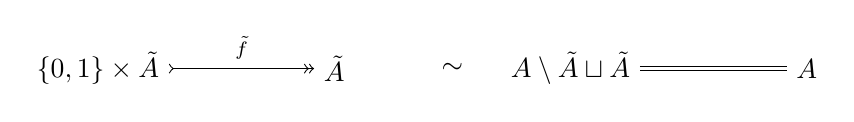
\begin{tikzpicture}[auto]
    \node (a) at (0, 0) {$\left\{ 0,1\right\} \times \tilde{A} $};
    \node (b) at (3, 0) {$\tilde{A} $};
    \node (c) at (6, 0) {$A\setminus \tilde{A} \sqcup \tilde{A} $};
    \node (d) at (9, 0) {$A$};
    \node (e) at (4.5, 0) {$\sim $};
    \draw [>->>] (a) to node {$\scriptstyle \tilde{f} $} (b);
    \draw [double distance=1pt] (c) to node {$\scriptstyle $} (d);
  \end{tikzpicture} 
\end{center}
次式のようになる。
\begin{align*}
\# A &= \# {A \setminus \widetilde{A} \sqcup \widetilde{A}}\\
&= \# \widetilde{A}\\
&= \# {\left\{ 0,1 \right\} \times \widetilde{A}}\\
&= \# \left\{ 0,1 \right\}\# \widetilde{A}\\
&= 2\# \widetilde{A}\\
&= 2\# {A \setminus \widetilde{A} \sqcup \widetilde{A}}\\
&= 2\# A
\end{align*}
ここで、$\# B \leq \# A$が成り立つなら、次式が成り立つことにより、
\begin{align*}
\# A &\leq \# A + \# B\\
&\leq \# A + \# A\\
&= 2\# A
\end{align*}
$\# A + \# B = \# A$が成り立つ。\par
その集合$A$の部分集合$A'$とこれを用いた全単射な写像$f:A' \times A'\overset{\sim}{\rightarrow}A'$の組$\left( A',f \right)$が考えられるとする。このとき、その集合$A'$が可算集合である、即ち、$\# A' = \aleph_{0}$が成り立つとき、定理\ref{1.2.7.7}より$\# \left( A' \times A' \right) = \aleph_{0}$が成り立つ、即ち、$\aleph_{0}^{2} = \aleph_{0}$が成り立つので、そのような写像$f$は存在しその組$\left( A',f \right)$は存在する。\par
ここで、そのような組$\left( A',f \right)$全体の集合を$\mathfrak{M}$とおく。その集合$\mathfrak{M}$の任意の2つの元々$\left( A',f \right)$、$\left( B',g \right)$を用いて$A' \subseteq B'$かつ$g|A' \times A' = f$が成り立つことが$\left( A',f \right)O\left( B',g \right)$と定義されるとする。このとき、上記と同様にして、その組$\left( \mathfrak{M,}O \right)$が帰納的な順序集合であることが示される。\par
したがって、Zornの補題よりその集合$\mathfrak{M}$には極大元$\left( \widetilde{A},\widetilde{f} \right)$が存在する。上記と同様にして、$\# \widetilde{A} \geq \aleph_{0}$が成り立つことが示される。ここで、$\# {A \setminus \widetilde{A}} \geq \# \widetilde{A}$が成り立つと仮定すると、$A'' \sim \widetilde{A}$なるその集合$A \setminus \widetilde{A}$の部分集合$A''$が存在するのであった。したがって、次のようになり、
\begin{align*}
\left( \widetilde{A} \sqcup A'' \right) \times \left( \widetilde{A} \sqcup A'' \right) &= \left( \left( \widetilde{A} \sqcup A'' \right) \times \widetilde{A} \right) \sqcup \left( \left( \widetilde{A} \sqcup A'' \right) \times A'' \right)\\
&= \left( \widetilde{A} \times \widetilde{A} \right) \sqcup \left( A'' \times \widetilde{A} \right) \sqcup \left( \widetilde{A} \times A'' \right) \sqcup \left( A'' \times A'' \right)
\end{align*}
ここで、次式が成り立つので、
\begin{align*}
\widetilde{A} \sim \widetilde{A} \times \widetilde{A} \sim A'' \times \widetilde{A} \sim \widetilde{A} \times A'' \sim A'' \times A''
\end{align*}
したがって、その集合$\left( A'' \times \widetilde{A} \right) \sqcup \left( \widetilde{A} \times A'' \right) \sqcup \left( A'' \times A'' \right)$を$D$とおくと、次式のようになる。
\begin{align*}
\# D &= \# {\left( A'' \times \widetilde{A} \right) \sqcup \left( \widetilde{A} \times A'' \right) \sqcup \left( A'' \times A'' \right)}\\
&= \# {A'' \times \widetilde{A}} + \# {\widetilde{A} \times A''} + \# {A'' \times A''}\\
&= \# \widetilde{A} + \# \widetilde{A} + \# \widetilde{A}\\
&= 3\# \widetilde{A} = \# \widetilde{A}
\end{align*}
これにより、全単射$g:D\overset{\sim}{\rightarrow}A''$が存在し、次式のような写像$g'$が定義されると、
\begin{align*}
g':\left( \widetilde{A} \sqcup A'' \right) \times \left( \widetilde{A} \sqcup A'' \right) \rightarrow \widetilde{A} \sqcup A'';a \mapsto \left\{ \begin{matrix}
\widetilde{f}(a) & \mathrm{if} & a \in \widetilde{A} \times \widetilde{A} \\
g(a) & \mathrm{if} & a \in D \\
\end{matrix} \right.\ 
\end{align*}
次式が成り立つことにより、
\begin{align*}
\left( \widetilde{A} \sqcup A'' \right) \times \left( \widetilde{A} \sqcup A'' \right) = \left( \widetilde{A} \times \widetilde{A} \right) \sqcup D
\end{align*}
その写像$g$は全単射である。以上より、$\widetilde{A} \subset \widetilde{A} \sqcup A''$かつ$g'|\widetilde{A} \times \widetilde{A} = \widetilde{f}$が成り立つので、$\left( \widetilde{A},\widetilde{f} \right)O\left( \widetilde{A} \sqcup A'',g' \right)$が成り立つことになる。しかしながら、これはその組$\left( \widetilde{A},\widetilde{f} \right)$がその集合$\mathfrak{M}$の極大元であることに矛盾する。したがって、$\# \left( A \setminus \widetilde{A} \right) < \# \widetilde{A}$が成り立つ。\par
したがって、上記の議論により次式のようになり、
\begin{center}
  \begin{tikzpicture}[auto] 
    \node (a) at (0, 0) {$\tilde{A} \times \tilde{A} $};
    \node (b) at (3, 0) {$\tilde{A} $};
    \node (c) at (6, 0) {$A\setminus \tilde{A} \sqcup \tilde{A} $};
    \node (d) at (9, 0) {$A$};
    \node (e) at (4.5, 0) {$\sim $};
    \draw [>->>] (a) to node {$\scriptstyle \tilde{f} $} (b);
    \draw [double distance=1pt] (c) to node {$\scriptstyle $} (d);  
  \end{tikzpicture} 
\end{center}
次のようになる。
\begin{align*}
\# A &= \# {\widetilde{A} \sqcup A \setminus \widetilde{A}}\\
&= \# \widetilde{A} + \# {A \setminus \widetilde{A}}\\
&= \# \widetilde{A}\\
&= \# {\widetilde{A} \times \widetilde{A}}\\
&= \# \widetilde{A}\# \widetilde{A}\\
&= {\# \widetilde{A}}^{2}\\
&= \left( \# \widetilde{A} + \# {A \setminus \widetilde{A}} \right)^{2}\\
&= \left( \# {\widetilde{A} \sqcup A \setminus \widetilde{A}} \right)^{2}\\
&= \left( \# A \right)^{2}
\end{align*}
ここで、$1 \leq \# B \leq \# A$が成り立つなら、次式が成り立つことにより、
\begin{align*}
\# A &\leq \# A\# B\\
&\leq \# A\# A\\
&= \left( \# A \right)^{2}
\end{align*}
$\# A\# B = \# A$が成り立つ。\par
$2 \leq \# B \leq \# A$が成り立つなら、$2^{\# A} \leq {\# B}^{\# A}$が成り立つ。ここで、$\# B < \# {\mathfrak{P}(B)}$が成り立つので、次のようになる。
\begin{align*}
{\# B}^{\# A} &\leq {\# {\mathfrak{P}(B)}}^{\# A}\\
&= \left( 2^{\# B} \right)^{\# A}\\
&= 2^{\# A\# B}
\end{align*}
ここで、$\# A\# B = \# A$が成り立つので、したがって、$2^{\# A} = {\# B}^{\# A}$が成り立つ。
\end{proof}
\begin{thebibliography}{50}
  \bibitem{1}
    松坂和夫, 集合・位相入門, 岩波書店, 1968. 新装版第2刷 p97-115,125-129 ISBM978-4-00-029871-1
\end{thebibliography}
\end{document}
